\documentclass[onlytextwidth, aspectratio=169]{beamer}
\documentclass[onlytextwidth, aspectratio=169]{beamer}
\usepackage[utf8]{inputenc}
\usepackage{microtype}
\usepackage{amsmath}
\usepackage{amssymb}
\usepackage[nomessages]{fp} %\FPeval{\var-name}{2*sin(pi/6)}
\usepackage{siunitx} %units in math. eg 20\milli\meter
\usepackage{yhmath} % for arcs, overparenth command
\usepackage{tikz} %graphics
\usetikzlibrary{quotes, angles, arrows, arrows.meta}
%\usepackage{graphicx} already loaded by beamer class
%consider setting \graphicspath{{images/}}
%\parskip ?? to avoid paragraph indent
\usepackage{multicol} %may not need this package, just columns environment
\usepackage{venndiagram}

\subtitle[BECA]{Bronx Early College Academy}
\author[Huson]{Christopher J. Huson PhD}

\setbeamertemplate{headline}{\vskip2mm 
  \, BECA / \insertshortauthor \, / \inserttitle
  \hfill 
  \insertsection
  }

%Tick mark commands
\newcommand\ticks{}
  \def\ticks{{Bar[scale=2]}-{Bar[scale=2]}}
\newcommand\paraticks{}
  \def\paraticks{{Straight Barb[reversed, scale=2]}-{Straight Barb[scale=2]}}

\title{Geometry Unit 9: Dilation and similarity}
\date{13 March 2023 - 31 March 2023}

\begin{document}
\frame{\titlepage}
\section[Outline]{}
\frame{\tableofcontents}

\section{9.1 Dilation introduction \hfill 13 March \,}
\begin{frame}{Learning Target: I can dilate a triangle}
  {HSG.SRT.B.5 Use similarity criteria for triangles to solve problems \hfill \alert{9.1 Monday 13 March}}
    Do Now
    \begin{enumerate}
      \item $12 \times \frac{1}{3}=$
      \item $10 \times \frac{7}{5}=$
      \item Find $x$ if $9 \cdot x = 15$
    \end{enumerate}
    Lesson: Dilation, transformations, fraction operations \\
    Test results, check Jumprope\\[0.5cm]
    Homework: Complete the classwork practice, Deltamath problem set
\end{frame}

\begin{frame}{A dilation centered at the origin with scale factor $k=2$}
  \begin{columns}
    \column{0.6\textwidth}
    $\triangle ABC \rightarrow \triangle A'B'C'$\\[0.2cm]
    $A(0,0) \rightarrow A'(0,0)$\\
    $B(2,1) \rightarrow B'(4,2)$\\
    $C(1,-1) \rightarrow C'(2,-2)$ \vspace{0.3cm}
      \begin{description}
        \item[Dilation] A transformation stretching objects on the plane by a scale factor away from a point
        \item[Center] Dilation stretches figures away from a stationary point, the ``center of dilation''
        \item[Scale factor] The ratio $k$ of the lengths of the corresponding sides of dilated figures
      \end{description}
    \column{0.4\textwidth}
    \begin{flushright}
      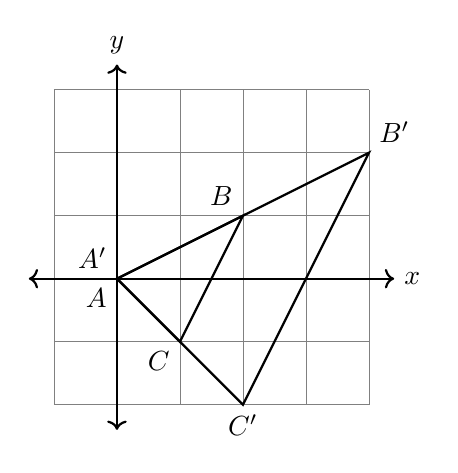
\begin{tikzpicture}[scale=0.8]
        \draw [help lines] (-1,-2) grid (4,3);
        \draw [thick, <->] (-1.4,0) -- (4.4,0) node [right] {$x$};
        \draw [thick, <->] (0,-2.4)--(0,3.4) node [above] {$y$};  
        \draw [thick]
          (0,0) node[below left] {$A$}--
          (2,1) node[above left] {$B$}--
          (1,-1) node[below left] {$C$}--cycle;
        \draw [thick]
          (0,0) node[above left] {$A'$}--
          (4,2) node[above right] {$B'$}--
          (2,-2) node[below] {$C'$}--cycle; 
      \end{tikzpicture}
    \end{flushright}
  \end{columns}
\end{frame}

\section{9.2 Solving for $k$, similarity \hfill 15 March \,}
\begin{frame}{Learning Target: I can identify and explain similarity}
  {HSG.SRT.B.5 Use similarity criteria for triangles to solve problems \hfill \alert{9.2 Wednesday 15 March}}
    Do Now: A triangle with side lengths 3, 4, and 5 is dilated by a factor of $k=2$ centered at one of its vertices. Find the lengths of the image's sides. \\[0.5cm]
    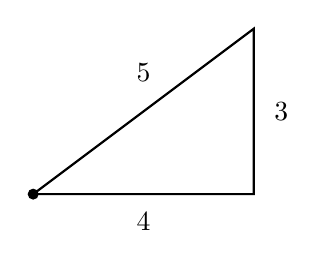
\begin{tikzpicture}[scale=0.7]
      \draw [thick] (0,0)--(4,0)--(4,3)--cycle;
      \node at (2,-0.5){4};
      \node at (2,2.2){5};
      \node at (4.5,1.5){3};
      \fill (0,0) circle[radius=0.1];
    \end{tikzpicture} \\[0.5cm]
    Lesson: Similar objects, solving for scale factor $k$ \\[0.5cm]
    Homework: Complete the classwork practice, Deltamath problem set \\[0.5cm]
\end{frame}

\begin{frame}{Similarity, corresponding parts, and scaled proportions}
  \begin{columns}
    \column{0.5\textwidth}
      \begin{description}
        \item[Similarity] Objects with the same shape, but not necessarily the same size, are similar. Their corresponding angles are congruent and their corresponding sides are proportional.
        \item[Notation] This is the symbol for similar triangles: $\triangle ABC \sim \triangle DEF$
        \item[Definition] Two figures are similar if one or more rigid motions and a dilation will carry one figure onto the other.
      \end{description}
    \column{0.5\textwidth}
    \begin{flushright}
      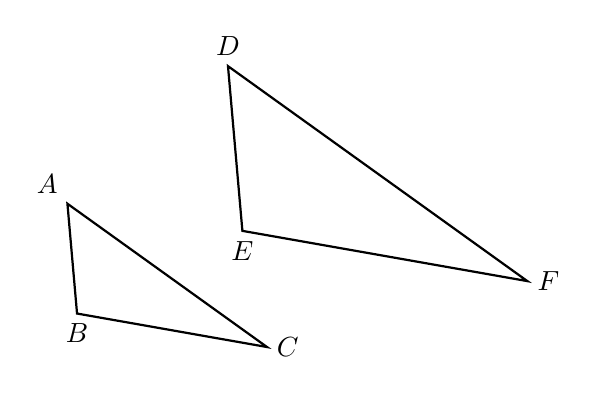
\begin{tikzpicture}[scale=0.7]
        \coordinate [label=above left:$A$](A) at (95:2);
        \coordinate [label=below:$B$](B) at (0, 0);
        \coordinate [label=right:$C$](C) at (-10:3.5);
        \draw [thick] (A)--(B)--(C)--cycle;
        \draw [thick, xshift=3cm, yshift=1.5cm, scale=1.5] 
          (95:2) node[above]{$D$}--
          (0,0) node[below]{$E$}--
          (-10:3.5) node[right]{$F$}--cycle;
      \end{tikzpicture}
    \end{flushright}
  \end{columns}
\end{frame}

\section{9.3 Overlapping triangle practice \hfill 16 March \,}
\begin{frame}{Learning Target: I can solve overlapping similar triangles}
  {HSG.SRT.B.5 Use similarity criteria for triangles to solve problems \hfill \alert{9.3 Thursday 16 March}}
  \begin{columns}
    \column{0.5\textwidth}
    Do Now: Given $\triangle ABC \sim \triangle DEF$, $k=2$ \\
    If $BC=4$, find $EF$ \\
    If m$\angle B = 80^\circ$, find m$\angle E$\\[0.5cm]
    Lesson: Flexibly applying similarity to situations \\[0.5cm]
    Homework: Complete the classwork practice, Deltamath problem set \\[0.5cm]
    \column{0.5\textwidth}
    \begin{flushright}
      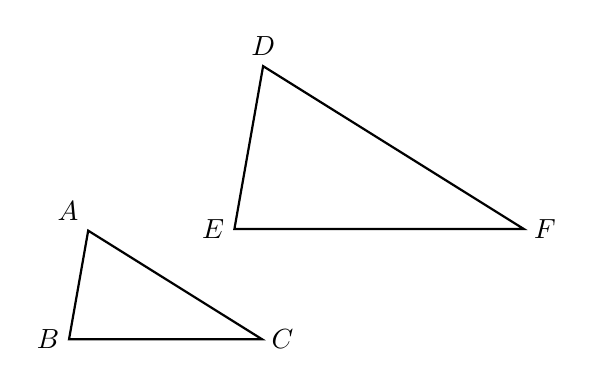
\begin{tikzpicture}[scale=0.7]
        \coordinate [label=above left:$A$](A) at (80:2);
        \coordinate [label=left:$B$](B) at (0, 0);
        \coordinate [label=right:$C$](C) at (0:3.5);
        \draw [thick] (A)--(B)--(C)--cycle;
        \draw [thick, xshift=3cm, yshift=2cm, scale=1.5] 
          (80:2) node[above]{$D$}--
          (0,0) node[left]{$E$}--
          (0:3.5) node[right]{$F$}--cycle;
      \end{tikzpicture}
    \end{flushright}
  \end{columns}
\end{frame}

\begin{frame}{``Solve'' a triangle by finding all of is sides' and angles' measures}
    Given $\triangle ABC \sim \triangle DEF$ \\[0.2cm]
    $BC=4$, $EF=6$, $AB=3$\\[0.2cm]
    m$\angle B = 55^\circ$, m$\angle D=70^\circ$\\[0.5cm]
    \begin{center}
      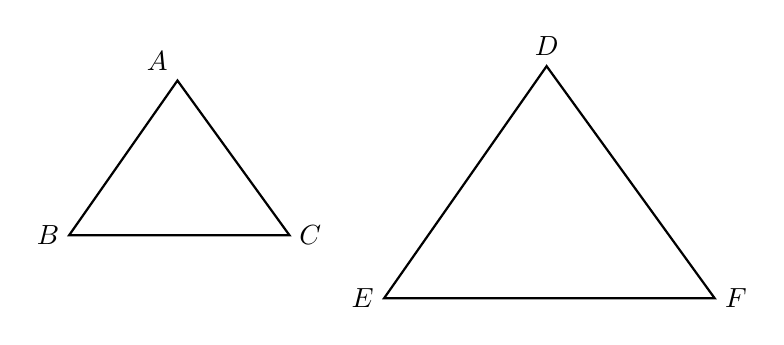
\begin{tikzpicture}[scale=0.8]
        \coordinate [label=above left:$A$](A) at (55:3);
        \coordinate [label=left:$B$](B) at (0, 0);
        \coordinate [label=right:$C$](C) at (0:3.5);
        \draw [thick] (A)--(B)--(C)--cycle;
        \draw [thick, xshift=5cm, yshift=-1cm, scale=1.5] 
          (55:3) node[above]{$D$}--
          (0,0) node[left]{$E$}--
          (0:3.5) node[right]{$F$}--cycle;
      \end{tikzpicture}
    \end{center}
\end{frame}

\begin{frame}{Apply a dilation centered at the origin with scale factor $k=\frac{1}{2}$}
  \begin{columns}
    \column{0.4\textwidth}
    $\triangle ABC \rightarrow \triangle A'B'C'$\\[0.5cm]
    $A(-2,0) \rightarrow$ \onslide<2>{\textcolor{red}{$A'(-1,0)$}}\\[0.5cm]
    $B(4,2) \rightarrow$ \onslide<2>{\textcolor{red}{$B'(2,1)$}}\\[0.5cm]
    $C(2,-4) \rightarrow$ \onslide<2>{\textcolor{red}{$C'(1,-2)$}}\\[0.5cm]
    \onslide<2>{Note:\\ Slope is invariant under dilation}
    \column{0.6\textwidth}
    \begin{flushright}
      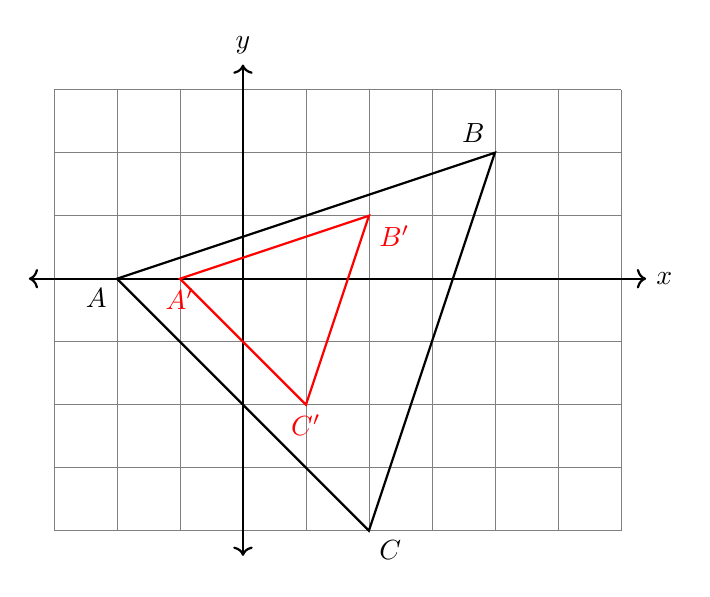
\begin{tikzpicture}[scale=0.8]
        \draw [help lines] (-3,-4) grid (6,3);
        \draw [thick, <->] (-3.4,0) -- (6.4,0) node [right] {$x$};
        \draw [thick, <->] (0,-4.4)--(0,3.4) node [above] {$y$};  
        \draw [thick]
          (-2,0) node[below left] {$A$}--
          (4,2) node[above left] {$B$}--
          (2,-4) node[below right] {$C$}--cycle;
        \pause
          \draw [thick, red]
          (-1,0) node[below] {$A'$}--
          (2,1) node[below right] {$B'$}--
          (1,-2) node[below] {$C'$}--cycle; 
      \end{tikzpicture}
    \end{flushright}
  \end{columns}
\end{frame}

\section{9.4 Composition \hfill 17 March \,}
\begin{frame}{Learning Target: I can compose dilations with other transformations}
  {HSG.SRT.B.5 Use similarity criteria for triangles to solve problems \hfill \alert{9.4 Friday 17 March}}
  \begin{columns}
    \column{0.4\textwidth}
    Do Now:\\
    First reflect $\triangle ABC$ over the $y$-axis \\
    Then slide it up one and the right 3 \\[0.5cm]
    Lesson: Applying dilation and rigid motions in compositions \\[0.5cm]
    Homework: Complete the classwork practice, Deltamath problem set \\[0.5cm]
    \column{0.6\textwidth}
    \begin{flushright}
      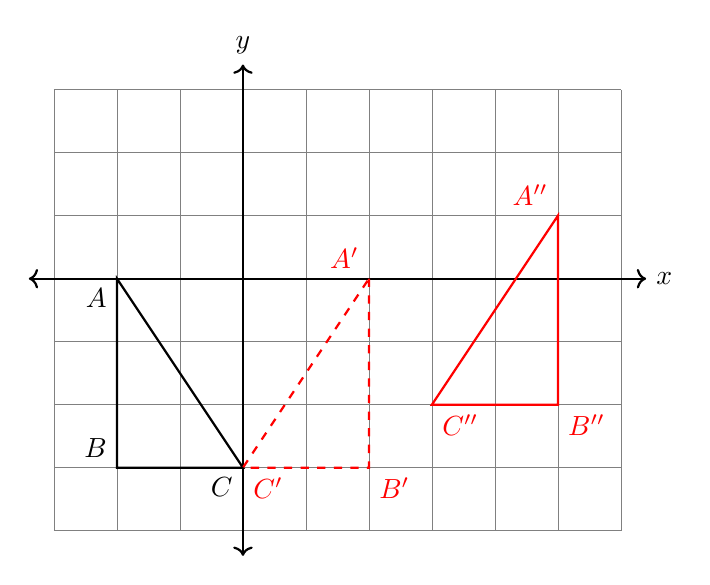
\begin{tikzpicture}[scale=0.8]
        \draw [help lines] (-3,-4) grid (6,3);
        \draw [thick, <->] (-3.4,0) -- (6.4,0) node [right] {$x$};
        \draw [thick, <->] (0,-4.4)--(0,3.4) node [above] {$y$};  
        \draw [thick]
          (-2,0) node[below left] {$A$}--
          (-2,-3) node[above left] {$B$}--
          (0,-3) node[below left] {$C$}--cycle;
        \pause
          \draw [thick, red, dashed]
            (2,0) node[above left] {$A'$}--
            (2,-3) node[below right] {$B'$}--
            (0,-3) node[below right] {$C'$}--cycle;
          \draw [thick, red]
            (5,1) node[above left] {$A''$}--
            (5,-2) node[below right] {$B''$}--
            (3,-2) node[below right] {$C''$}--cycle; 
      \end{tikzpicture}
    \end{flushright}
  \end{columns}
\end{frame}

\begin{frame}{Find the area of the large and small rectangles}
  {(use the areas of the small triangles)}
    \begin{flushright}
      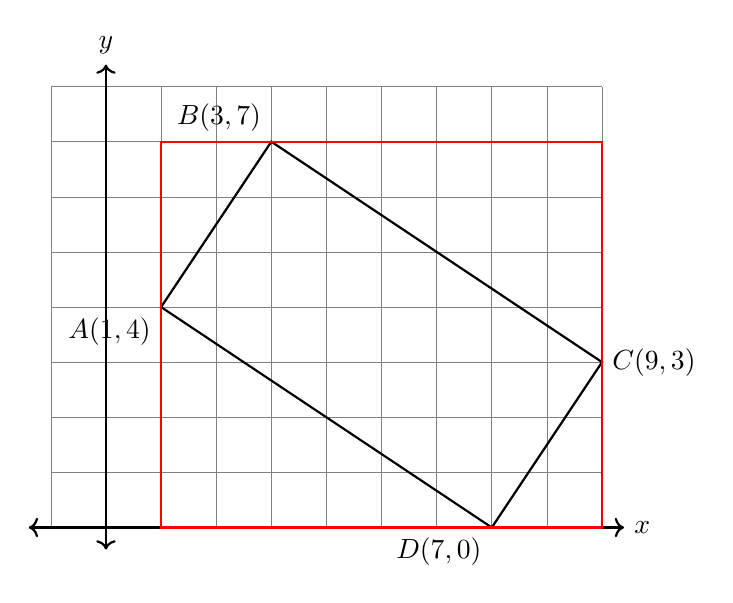
\begin{tikzpicture}[scale=0.7]
        \draw [help lines] (-1,0) grid (9,8);
        \draw [thick, <->] (-1.4,0) -- (9.4,0) node [right] {$x$};
        \draw [thick, <->] (0,-0.4)--(0,8.4) node [above] {$y$};  
        \draw [thick]
          (1,4) node[below left] {$A(1,4)$}--
          (3,7) node[above left] {$B(3,7)$}--
          (9,3) node[right] {$C(9,3)$}--
          (7,0) node[below left] {$D(7,0)$}--cycle;
        \draw [thick, red] (1,7)--(9,7)--(9,0)--(1,0)--cycle;
      \end{tikzpicture}
    \end{flushright}
\end{frame}

\section{9.5 Composition \hfill 21 March \,}
\begin{frame}{Learning Target: I can compose dilations with other transformations}
  {HSG.SRT.B.5 Use similarity criteria for triangles to solve problems \hfill \alert{9.5 Tuesday 21 March}}
  \begin{columns}
    \column{0.4\textwidth}
    Do Now:\\
    First reflect $\triangle ABC$ over the $y$-axis \\
    Then slide it up one and the right 3 \\[0.5cm]
    Lesson: Applying dilation and rigid motions in compositions \\[0.5cm]
    Homework: Complete the classwork practice, Deltamath problem set \\[0.5cm]
    \column{0.6\textwidth}
    \begin{flushright}
      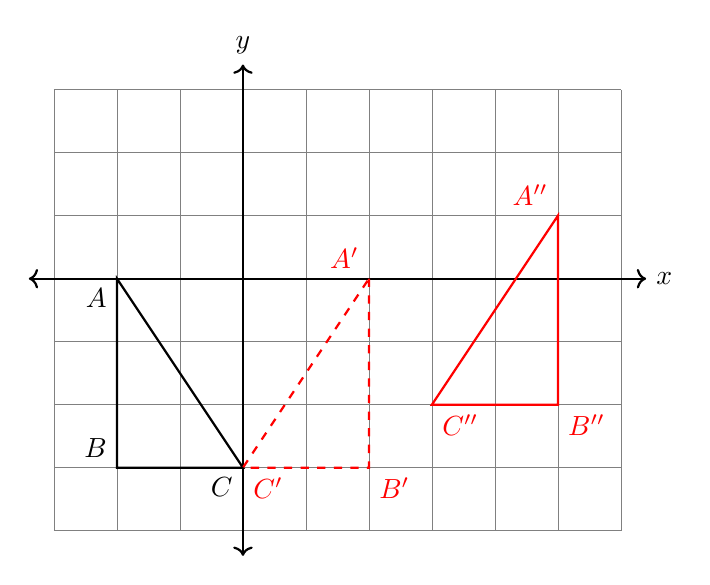
\begin{tikzpicture}[scale=0.8]
        \draw [help lines] (-3,-4) grid (6,3);
        \draw [thick, <->] (-3.4,0) -- (6.4,0) node [right] {$x$};
        \draw [thick, <->] (0,-4.4)--(0,3.4) node [above] {$y$};  
        \draw [thick]
          (-2,0) node[below left] {$A$}--
          (-2,-3) node[above left] {$B$}--
          (0,-3) node[below left] {$C$}--cycle;
        \pause
          \draw [thick, red, dashed]
            (2,0) node[above left] {$A'$}--
            (2,-3) node[below right] {$B'$}--
            (0,-3) node[below right] {$C'$}--cycle;
          \draw [thick, red]
            (5,1) node[above left] {$A''$}--
            (5,-2) node[below right] {$B''$}--
            (3,-2) node[below right] {$C''$}--cycle; 
      \end{tikzpicture}
    \end{flushright}
  \end{columns}
\end{frame}

\section{9.6 Midline and medians \hfill 22 March \,}
\begin{frame}{Learning Target: I can plot triangle midlines and medians}
  {HSG.SRT.B.5 Use similarity criteria for triangles to solve problems \hfill \alert{9.6 Wednesday 22 March}}
  \begin{columns}
    \column{0.4\textwidth}
    Do Now:\\
    Rotating the triangle around its longer leg will make what 3-dimensional shape? \\[0.5cm]
    Lesson: Regents pointers. Be on time tomorrow. \\[0.5cm]
    Homework: Complete the classwork practice, Deltamath problem set \\[0.5cm]
    \column{0.6\textwidth}
    \begin{flushright}
      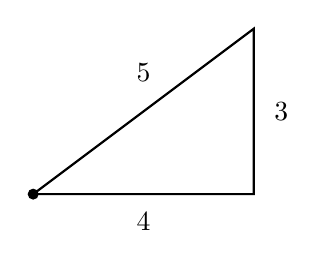
\begin{tikzpicture}[scale=0.7]
        \draw [thick] (0,0)--(4,0)--(4,3)--cycle;
        \node at (2,-0.5){4};
        \node at (2,2.2){5};
        \node at (4.5,1.5){3};
        \fill (0,0) circle[radius=0.1];
      \end{tikzpicture}
    \end{flushright}
  \end{columns}
\end{frame}

\section{9.7 Midline and medians \hfill 24 March \,}
\begin{frame}{Learning Target: I can plot triangle midlines and medians}
  {HSG.SRT.B.5 Use similarity criteria for triangles to solve problems \hfill \alert{9.7 Friday 24 March}}
  \begin{columns}
    \column{0.4\textwidth}
    Do Now:\\
    What sequence of transformations map similar triangles $\triangle ABP \rightarrow \triangle JKP$? \\[0.5cm]
    Lesson: Midlines and triangle medians \\[0.5cm]
    Homework: Complete the classwork practice, Deltamath problem set \\[0.5cm]
    \column{0.6\textwidth}
    \begin{flushright}
      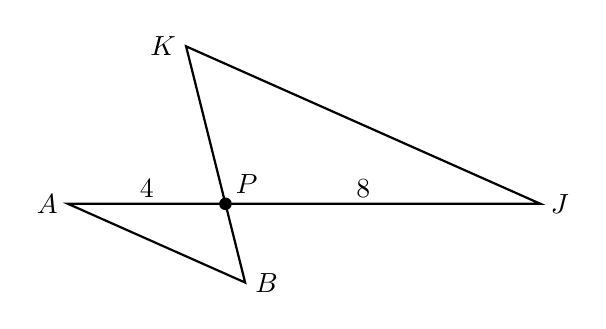
\begin{tikzpicture}[scale=1.0]
          \draw [thick]
            (0.25,-1)node[right]{$B$}--
            (-0.5,2)node[left]{$K$}--
            (4,0)node[right]{$J$}--
            (0,0)node[above right]{$P$}--
            (-2,0)node[left]{$A$}--cycle;
          \fill (0,0) circle (0.08);
          \node at (-1,0.2) {$4$};
          \node at (1.75,0.2) {$8$};
        \end{tikzpicture}
    \end{flushright}
  \end{columns}
\end{frame}

\begin{frame}{Triangle midline and medians create similar triangles}
  \begin{columns}
    \column{0.6\textwidth}
      \begin{description}
        \item[Midpoint] The point on a segment that divides the segment into two equal parts.
        \item[Midline] The line segment that connects the midpoints of two sides of a triangle.
        \onslide<2>{\item[Medians] Segments connecting a vertex to the midpoint of the opposite side.
        \item[Centroid] The point where the three medians intersect.}
      \end{description}
    \column{0.4\textwidth}
    \begin{flushright}
      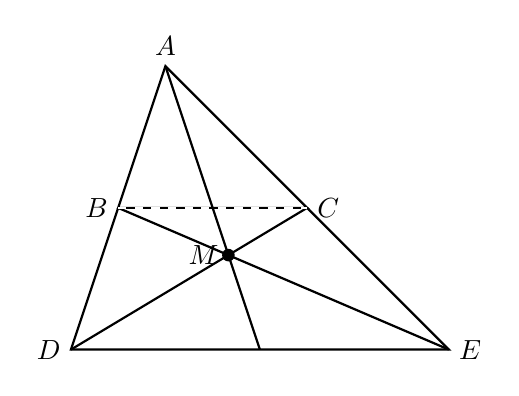
\begin{tikzpicture}[scale=0.4]
        \draw [thick]
        (0.5,1.5)node[left]{$B$}--
        (6.5,1.5)node[right]{$C$}--
        (2,6)node[above]{$A$}--cycle;
        \draw [thick] (0.5,1.5)--
          (-1,-3)node[left]{$D$}--
          (11,-3)node[right]{$E$}--(6.5,1.5);
        \pause
          \draw [thick] (2,6)--(5,-3);
          \draw [thick] (0.5,1.5)--(11,-3);
          \draw [thick] (6.5,1.5)--(-1,-3);
          \fill (4,0) circle (0.2)node[left]{$M$};
          \draw [dashed, thick, white] (0.5,1.5)--(6.5,1.5);
        %\node at (3,2.5)[below]{$7$};
        %\node at (2.1, 0)[above]{$4$};
        %\node at (-0.7, -1)[above]{$5$};
      \end{tikzpicture}
    \end{flushright}
  \end{columns}
\end{frame}

\section{9.8 Scaling \hfill 29 March \,}
\begin{frame}{Learning Target: I can scale area and perimeter}
  {HSG.SRT.B.5 Use similarity criteria for triangles to solve problems \hfill \alert{9.8 Wednesday 29 March}}
  \begin{columns}
    \column{0.4\textwidth}
    Do Now:\\
    What sequence of transformations map similar triangles $\triangle ABP \rightarrow \triangle JKP$? \\[0.5cm]
    Lesson: Scale factor $k$, area scales by $k^2$, volume by $k^3$ \\[0.5cm]
    Homework: Complete the classwork practice, Deltamath problem set \\[0.5cm]
    \column{0.6\textwidth}
    \begin{flushright}
      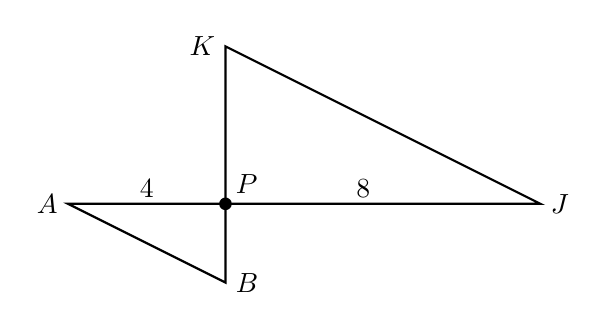
\begin{tikzpicture}[scale=1.0]
          \draw [thick]
            (0,-1)node[right]{$B$}--
            (0,2)node[left]{$K$}--
            (4,0)node[right]{$J$}--
            (0,0)node[above right]{$P$}--
            (-2,0)node[left]{$A$}--cycle;
          \fill (0,0) circle (0.08);
          \node at (-1,0.2) {$4$};
          \node at (1.75,0.2) {$8$};
        \end{tikzpicture}
    \end{flushright}
  \end{columns}
\end{frame}


\section{9.9 Scaling \hfill 30 March \,}
\begin{frame}{Learning Target: I can prove triangles similar using $AA$ similarity}
  {HSG.SRT.B.5 Use similarity criteria for triangles to solve problems \hfill \alert{9.9 Thursday 30 March}}
    Do Now:\\
    Given $\triangle ABC \sim \triangle XYZ$, m$\angle A = 50^\circ$, m$\angle Y = 60^\circ$ \\[0.25cm]
    Find the remaining angle measures. \\[0.5cm]
    Lesson: Triangles with congruent corresponding angles are similar \\[0.5cm]
    Homework: Complete the classwork practice, Deltamath problem set \\[0.5cm]
\end{frame}

\begin{frame}{Triangle midline and medians create similar triangles}
  \begin{columns}
    \column{0.6\textwidth}
      \begin{description}
        \item[Midpoint] The point on a segment that divides the segment into two equal parts.
        \item[Midline] The line segment that connects the midpoints of two sides of a triangle.
        \onslide<2>{\item[Medians] Segments connecting a vertex to the midpoint of the opposite side.
        \item[Centroid] The point where the three medians intersect.}
      \end{description}
    \column{0.4\textwidth}
    \begin{flushright}
      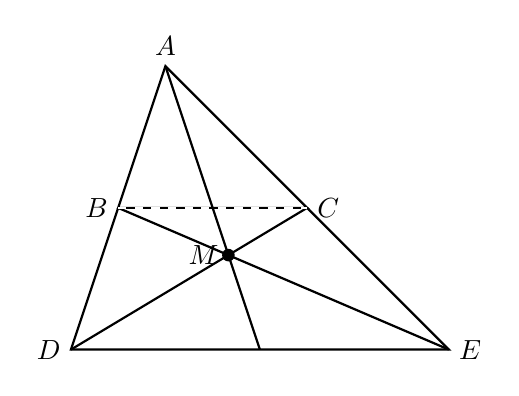
\begin{tikzpicture}[scale=0.4]
        \draw [thick]
        (0.5,1.5)node[left]{$B$}--
        (6.5,1.5)node[right]{$C$}--
        (2,6)node[above]{$A$}--cycle;
        \draw [thick] (0.5,1.5)--
          (-1,-3)node[left]{$D$}--
          (11,-3)node[right]{$E$}--(6.5,1.5);
        \pause
          \draw [thick] (2,6)--(5,-3);
          \draw [thick] (0.5,1.5)--(11,-3);
          \draw [thick] (6.5,1.5)--(-1,-3);
          \fill (4,0) circle (0.2)node[left]{$M$};
          \draw [dashed, thick, white] (0.5,1.5)--(6.5,1.5);
        %\node at (3,2.5)[below]{$7$};
        %\node at (2.1, 0)[above]{$4$};
        %\node at (-0.7, -1)[above]{$5$};
      \end{tikzpicture}
    \end{flushright}
  \end{columns}
\end{frame}

\begin{frame}{Notebook check scoring}
  {Start quickly at the beginning of class: notebook, pencil, folder, calculator; get to work}
    Jumprope mastery score
    \begin{enumerate}
      \item I have a notebook $\rightarrow$ 1
      \item I have class notes $\rightarrow$ 2
      \item I have stars indicating I quickly sit down and write the learning target $\rightarrow$ 3
      \item I have stars and I complete the Do Now right away $\rightarrow$ 4
    \end{enumerate} \bigskip
\end{frame}

\end{document}
